\beginsong{Auf vielen Straßen}[
    txt={Björn Behnke}, 
    mel={Alf Zschiesche},
    meljahr={1950}, 
    bo={34}, 
    gruen={47}, 
    siru={26},
    tonspur={154},
]

\beginverse
\endverse
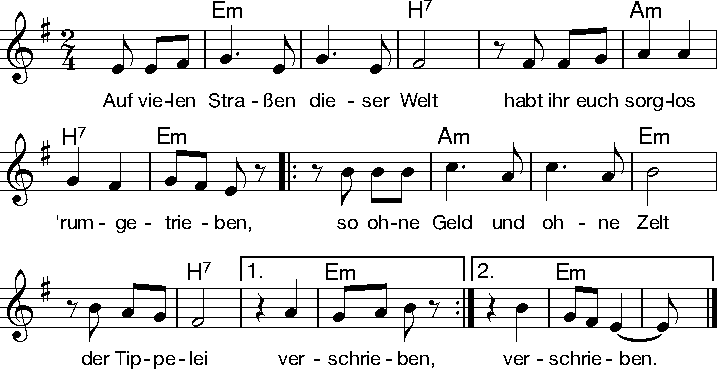
\includegraphics[draft=false, width=1\textwidth]{Noten/Lied006.pdf}	

\beginverse
Was galt euch \[Em]Armut, was Ge\[H7]fahr?
Ihr habt ver\[Am]achtet \[H7]und zer\[Em]schunden,
\lrep da draußen \[Am]treibend Jahr für \[Em]Jahr
doch euer \[H7]Glück ge\[Em]funden. \rrep
\endverse

\beginverse
Habt manches ^Lied der Einsam^keit
wohl in die ^Nacht hin^aus ge^sungen.
\lrep Auf fremden ^Meeren, fern der ^Zeit,
ist euer ^Sang ver^klungen. \rrep
\endverse

\endsong
